\chapter{Практическая Часть}
В данной части представлен листинг и результат работы программы.
\section{Листинг программы}
\begin{lstlisting}
function lab2()
X = [11.89,9.60,9.29,10.06,9.50,8.93,9.58,6.81,8.69,9.62,9.01,
10.59,10.50,11.53,9.94,8.84,8.91,6.90,9.76,7.09,11.29,11.25,
10.84,10.76,7.42,8.49,10.10,8.79,11.87,8.77,9.43,12.41,9.75,
8.53,9.72,9.45,7.20,9.23,8.93,9.15,10.19,9.57,11.09,9.97,8.81,
10.73,9.57,8.53,9.21,10.08,9.10,11.03,10.10,9.47,9.72,9.60,8.21,
7.78,10.21,8.99,9.14,8.60,9.14,10.95,9.33,9.98,9.09,10.35,8.61,
9.35,10.04,7.85,9.64,9.99,9.65,10.89,9.08,8.60,7.56,9.27,10.33,
10.09,8.51,9.86,9.24,9.63,8.67,8.85,11.57,9.85,9.27,9.69,10.90,
8.84,11.10,8.19,9.26,9.93,10.15,8.42,9.36,9.93,9.11,9.07,7.21,
8.22,9.08,8.88,8.71,9.93,12.04,10.41,10.80,7.17,9.00,9.46,10.42,
10.43,8.38,9.01];

    N = 1:length(X);
    
    gamma = 0.9;
    alpha = (1 - gamma)/2;

    mu = expectation(X);
    sSqr = variance(X); 

    fprintf('mu = %.4f\n', mu); 
    fprintf('S^2 = %.4f\n\n', sSqr);

    muArray = expectationArray(X, N);
    varArray = varianceArray(X, N);
 
    figure
    plot([N(1), N(end)], [mu, mu], 'm');
    hold on;
    plot(N, muArray, 'g');
\end{lstlisting}

\newpage
\begin{lstlisting}
     Ml = muArray - sqrt(varArray./N).*tinv(1 - alpha, N - 1);
    plot(N, Ml, 'b');

    fprintf('mu_low = %.4f\n', Ml(end));
    
    Mh = muArray + sqrt(varArray./N).*tinv(1 - alpha, N - 1);
    plot(N, Mh, 'r'), legend('y=mu', 'y=mu_n', 'y=mu-low_n', 'y=mu-high_n');
    grid on;
    hold off;
    
    fprintf('mu_high = %.4f\n', Mh(end));

    figure
    plot([N(1), N(end)], [sSqr, sSqr], 'm');
    hold on;
    plot(N, varArray, 'g');
    
    Sl = varArray.*(N - 1)./chi2inv(1 - alpha, N - 1);
    plot(N, Sl, 'b');
    
    Sh = varArray.*(N - 1)./chi2inv(alpha, N - 1);
    plot(N, Sh, 'r'), legend('z=S^2', 'z=S^2_n', 'z=S^2-low_n', 'z=S^2-high_n');
    grid on;
    hold off;

	
    fprintf('sigma^2_low = %.4f\n', Sl(end));
    fprintf('sigma^2_high = %.4f\n', Sh(end));
end

function mu = expectation(X)
   mu = mean(X);
end

function sSqr = variance(X)
    sSqr = var(X);
end
\end{lstlisting}
\newpage
\begin{lstlisting}
    function muArray = expectationArray(X, N)
    muArray = zeros(1, length(N));
    for i = 1:length(N)
        muArray(i) = expectation(X(1:N(i)));
    end
end

function varArray = varianceArray(X, N)
    varArray = zeros(1, length(N));
    for i = 1:length(N)
        varArray(i) = variance(X(1:N(i)));
    end
end
\end{lstlisting}

\section{Результаты работы программы}

\begin{equation*}
    \begin{split}
        &\hat{\mu} = 9.4872\\
        &S^2 = 1.2173\\
        &\underline{\mu} = 9.3202\\
        &\overline{\mu} = 9.6541\\
        &\underline{\sigma^2} = 0.9959\\
        &\overline{\sigma^2} = 1.5279\\
    \end{split}
\end{equation*}
\newpage

\section{Графики}
Построение на координатной плоскости $O_{yn}$ прямой $y=\hat{\mu}(\vec{x}_N)$, а также графиков функций $y=\hat{\mu}(\vec{x}_n)$, $y=\underline{\mu}(\vec{x}_n)$ и $\overline{\mu}(\vec{x}_n)$ как функций объема $n$ выборки, где $n$ изменяется от 1 до $N$;
\begin{figure}[h!]
    \centering
    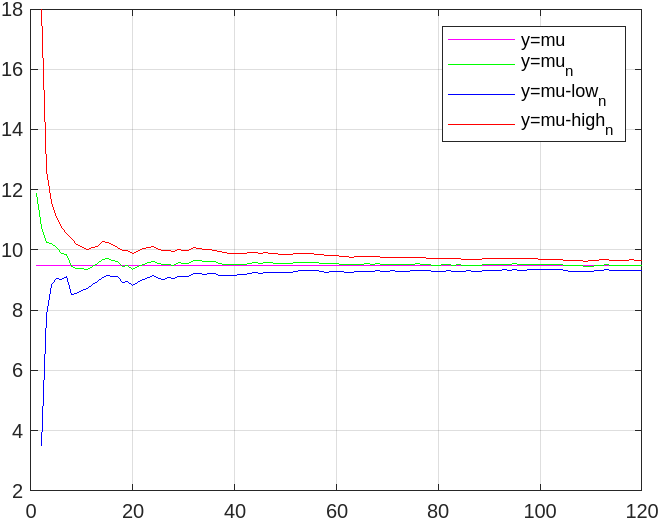
\includegraphics[]{images/lab_2_first.png}
    \caption{График для $\mu$}
\end{figure}
\newpage
Построение на другой координатной плоскости $O_{zn}$ прямой $z=S^2(\vec{x}_n)$, а также графиков функций $z=S^2(\vec{x}_N)$, $z=\underline{\sigma^2}(\vec{x}_n)$ и $\overline{\sigma^2}(\vec{x}_n)$ как функций объема $n$ выборки, где $n$ изменяется от 1 до $N$.
\begin{figure}[h!]
    \centering
    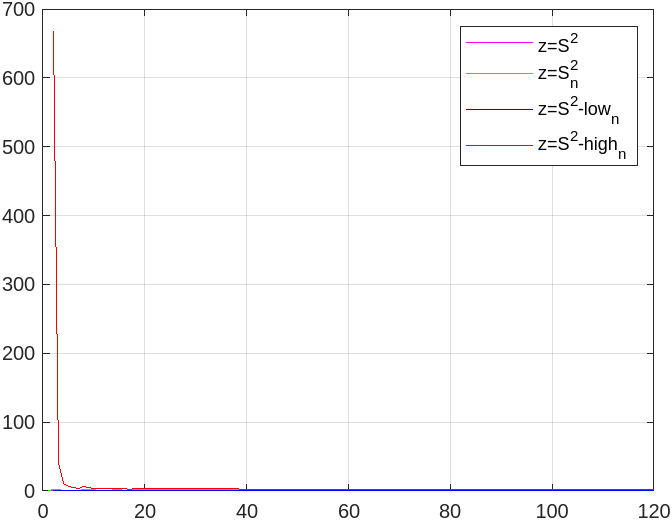
\includegraphics[]{images/lab_2_second.png}
    \caption{График для $\sigma$}
\end{figure}